\documentclass[../main.tex]{subfiles}
\begin{document}
\section{马尔可夫实时自定位计算}
$$p(\mathbf{x}_{t}|\mathbf{Z}^{t},\mathbf{U}^{t-1},\mathbf{m})=\eta p(\mathbf{z}_{t}|\mathbf{x}_{t},\mathbf{m})\int p(\mathbf{x}_{t}|\mathbf{x}_{t-1},\mathbf{u}_{t-1},\mathbf{m})p(\mathbf{x}_{t-1}|\mathbf{Z}^{t-1},\mathbf{U}^{t-2},\mathbf{m})d\mathbf{x}_{t-1}$$
\subsection{求解步骤}
\begin{itemize}
    \item 位姿预估 prediction(这里我们将这一项记作$\bar{p}$)
$$
\textcolor{red}{\bar{p}}(\mathbf{x}_{t}|\mathbf{Z}^{t},\mathbf{U}^{t-1},\mathbf{m})=\int p(\mathbf{x}_{t}|\mathbf{x}_{t-1},\mathbf{u}_{t-1},\mathbf{m})p(\mathbf{x}_{t-1}|\mathbf{Z}^{t-1},\mathbf{U}^{t-2},\mathbf{m})d\mathbf{x}_{t-1}$$
    \item 观测更新 updating
$$p(\mathbf{x}_{t}|\mathbf{Z}^{t},\mathbf{U}^{t-1},\mathbf{m})=\eta p(\mathbf{z}_{t}|\mathbf{x}_{t},\mathbf{m})\textcolor{red}{\bar{p}}(\mathbf{x}_{t}|\mathbf{Z}^{t},\mathbf{U}^{t-1},\mathbf{m})$$
\end{itemize}
{\small\kaishu{整个运算过于复杂,通常我们采用不同的假设或近似;一种方法是将非线性函数线性化(EKF),另一种方法是将连续函数离散化(PF)}}

\subsection{卡尔曼滤波定位方法(KF)}
\begin{enumerate}
    \item \textbf{前提条件}
        \begin{enumerate}
            \item 满足马尔可夫假设
            \item 运动(/状态转移)方程可表示为
$$\mathbf{x}_{t} = g(\mathbf{x}_{t-1}, \mathbf{u}_{t-1}) + \mathbf{v}_{t} ,\text{其中} \mathbf{v}_{t} \sim \mathcal{N}(0, \mathbf{R}_{t})$$
            \item 观测方程可表示为
$$
\mathbf{z}_{t} = h(\mathbf{x}_{t}) + \mathbf{\omega}_{t},\text{其中}\mathbf{\omega}_{t} \sim \mathcal{N}(0, \mathbf{Q}_{t})$$
            \item 初始位姿(/状态)概率 $p(\mathbf{x}_{0})$ 服从高斯分布
$$p(\mathbf{x}_{0}) = \mathcal{N}(\mathbf{x}_{0}; \boldsymbol{\mu}_{0}, 
\boldsymbol{\Sigma}_{0})$$
        \end{enumerate}
        若满足以上四个条件,则\textbf{状态估计的后验概率满足高斯分布}\footnote{这是因为若变量$x$服从高斯分布,经过线性变换后仍然服从高斯分布,即对高斯随机变量作任意线性转换,所得到的随机变量仍然满足高斯分布特性,其高斯分布参数能够用封闭形式求解},即$$p(\mathbf{x}_{t}) = \mathcal{N}(\mathbf{x}_{t}; \boldsymbol{\mu}_{t}, \boldsymbol{\Sigma}_{t})$$
        为求解$p(\mathbf{x}_{t})$,我们只需从$p(\mathbf{x}_{0})$开始递归计算均值和方差,最终得到$\boldsymbol{\mu}_{t}, \boldsymbol{\Sigma}_{t}$。
        \begin{figure}[H]
            \centering
            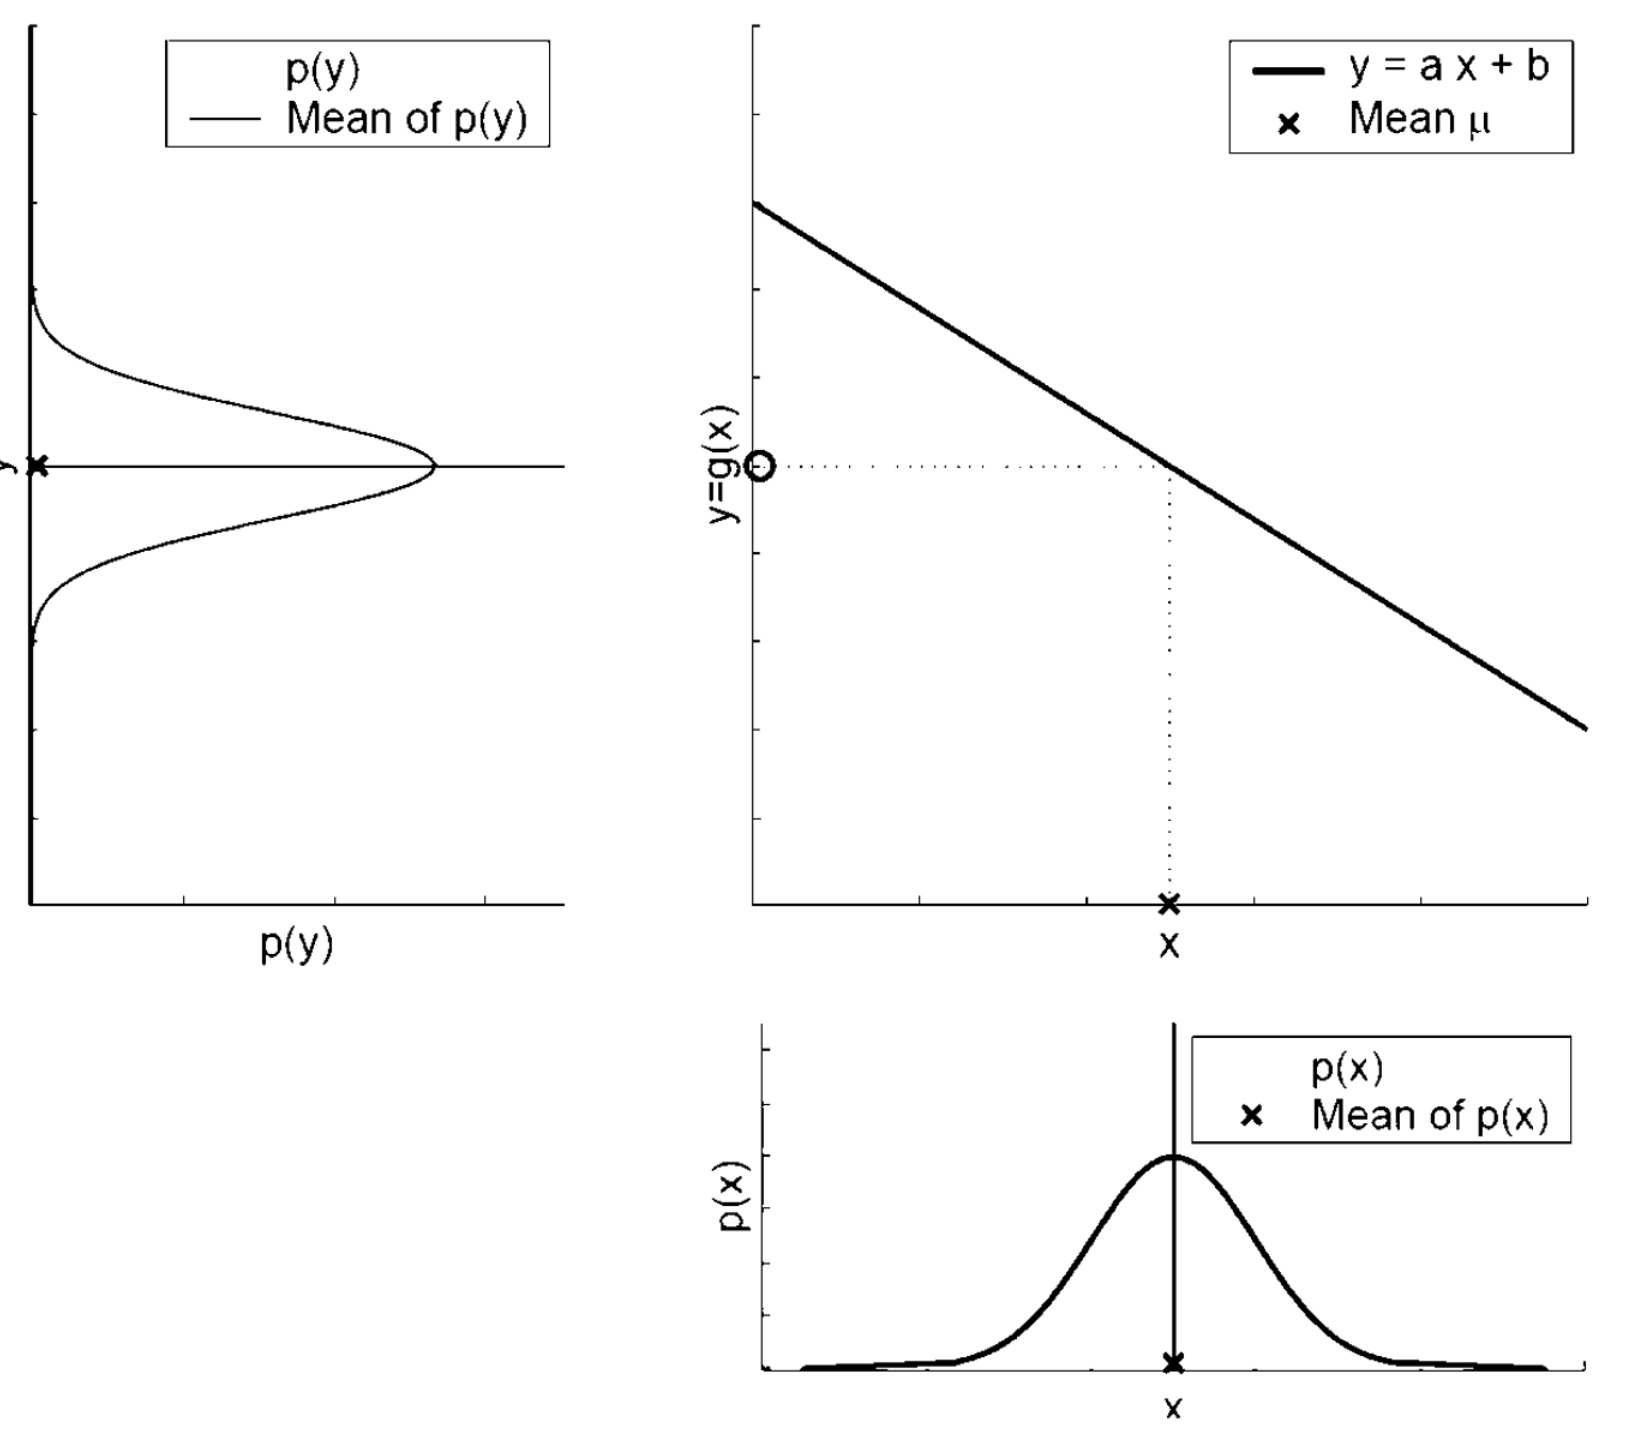
\includegraphics[width=0.4\linewidth]{images/linear.png}
            \caption{线性变换后的高斯分布}
        \end{figure}
        \item \textbf{Kalman filter算法公式}
          $$
          \bar{\boldsymbol{\mu}}_t = \mathbf{A}_t\boldsymbol{\mu}_{t-1} + \mathbf{B}_t\mathbf{u}_{t-1}
          $$
          $$
          \bar{\boldsymbol{\Sigma}}_t = \mathbf{A}_t\boldsymbol{\Sigma}_{t-1}\mathbf{A}_t^\top + \mathbf{R}_t
          $$
          则有:
          $$
          \mathbf{K}_t = \bar{\boldsymbol{\Sigma}}_t\mathbf{C}_t^\top\big(\mathbf{C}_t\bar{\boldsymbol{\Sigma}}_t\mathbf{C}_t^\top + \mathbf{Q}_t\big)^{-1}
          $$
          $$
          \boldsymbol{\mu}_t = \bar{\boldsymbol{\mu}}_t + \mathbf{K}_t\big(\mathbf{z}_t - \mathbf{C}_t\bar{\boldsymbol{\mu}}_t\big)
          $$
          $$
          \boldsymbol{\Sigma}_t = \big[\mathbf{I} - \mathbf{K}_t\mathbf{C}_t\big]\ \bar{\boldsymbol{\Sigma}}_t
          $$
          $$
          \text{return}\ \ \boldsymbol{\mu}_t,\ \boldsymbol{\Sigma}_t
          $$
          计算$\mathbf{K}_t$时,时间复杂度是$O(k^{2.376})$,其中$k$是特征向量维度,即观测到的特征数\\
          计算$\boldsymbol{\Sigma}_t$时,时间复杂度是$O(n^2)$,其中$n$是状态向量维度,即机器人的位姿描述维度
        \item \textbf{推导过程}
        {\small\kaishu{
        
\begin{enumerate}
  \item 运动方程(Motion model)
  
  $$\mathbf{x}_t = \mathbf{A}_t \mathbf{x}_{t-1} + \mathbf{B}_t \mathbf{u}_{t-1} + \mathbf{v}_t$$
  
  其中\\
  \begin{flushleft}
  $ \mathbf{x}_{t-1}\ \text{为}\ n\ \text{维向量,且}\ \mathbf{x}_{t-1}\sim\mathcal{N}(\boldsymbol{\mu}_{t-1},\boldsymbol{\Sigma}_{t-1})$\\
  $ \mathbf{u}_{t-1}\ \text{为}\ m\ \text{维向量}$\\
  $ \mathbf{v}_t\ \text{为}\ n\ \text{维向量,且}\ \mathbf{v}_t\sim\mathcal{N}(\mathbf{0},\mathbf{R}_t)$\\
  $ \mathbf{A}_t\ \text{为}\ n\times n\ \text{维矩阵}$\\
  $ \mathbf{B}_t\ \text{为}\ n\times m\ \text{维矩阵}$
  \end{flushleft}
    则有:
  $$p(\mathbf{x}_t\mid \mathbf{x}_{t-1},\mathbf{u}_{t-1})=\mathcal{N}\big(\mathbf{x}_t;\ \mathbf{A}_t\mathbf{x}_{t-1}+\mathbf{B}_t\mathbf{u}_{t-1},\ \mathbf{R}_t\big)$$

  \item 观测方程(Observation model)
  
  $$\mathbf{z}_t = \mathbf{C}_t \mathbf{x}_t + \boldsymbol{\omega}_t$$
  
  其中\\
  \begin{flushleft}
  $ \mathbf{C}_t\ \text{为}\ k\times n\ \text{维矩阵,且}\ k\ \text{为观测向量}\ \mathbf{z}_t\ \text{的维度}$\\
  $ \boldsymbol{\omega}_t\sim\mathcal{N}(\mathbf{0},\mathbf{Q}_t)$
  \end{flushleft}
则有:
  $$p(\mathbf{z}_t\mid \mathbf{x}_t)=\mathcal{N}\big(\mathbf{z}_t;\ \mathbf{C}_t\mathbf{x}_t,\ \mathbf{Q}_t\big)$$

  \item 状态预测(Prediction / Time update)
  
  $$\bar{p}(\mathbf{x}_t\mid \mathbf{Z}^{t-1},\mathbf{U}^{t-1})=\int p(\mathbf{x}_t\mid \mathbf{x}_{t-1},\mathbf{u}_{t-1})\;p(\mathbf{x}_{t-1}\mid \mathbf{Z}^{t-1},\mathbf{U}^{t-2})\ d\mathbf{x}_{t-1}$$
  
  $$p(\mathbf{x}_t\mid \mathbf{x}_{t-1},\mathbf{u}_{t-1})\sim\mathcal{N}\big(\mathbf{x}_t;\ \mathbf{A}_t\mathbf{x}_{t-1}+\mathbf{B}_t\mathbf{u}_{t-1},\ \mathbf{R}_t\big)$$
  
  $$p(\mathbf{x}_{t-1}\mid \mathbf{Z}^{t-1},\mathbf{U}^{t-2})\sim\mathcal{N}\big(\mathbf{x}_{t-1};\ \boldsymbol{\mu}_{t-1},\ \boldsymbol{\Sigma}_{t-1}\big)$$
  
  $$\bar{p}(\mathbf{x}_t\mid \mathbf{Z}^{t-1},\mathbf{U}^{t-1})=\mathcal{N}\big(\mathbf{x}_t;\ \bar{\boldsymbol{\mu}}_t,\ \bar{\boldsymbol{\Sigma}}_t\big)$$
  
  其中
  \begin{flushleft}
  $ \bar{\boldsymbol{\mu}}_t = \mathbf{A}_t\boldsymbol{\mu}_{t-1} + \mathbf{B}_t\mathbf{u}_{t-1}$\footnote{对前一时刻的均值做线性变换,不断加新的控制量}\\
  $ \bar{\boldsymbol{\Sigma}}_t = \mathbf{A}_t\boldsymbol{\Sigma}_{t-1}\mathbf{A}_t^\top + \mathbf{R}_t$\footnote{从公式可以看到很符合直觉的结论:对前一时刻的协方差做线性变换再加新的误差,所以里程估计不确定性越来越大}
  \end{flushleft}

  \item 观测更新(Measurement update / Correction)
  
  $$p(\mathbf{x}_t\mid \mathbf{Z}^t,\mathbf{U}^{t-1})=\eta\;p(\mathbf{z}_t\mid \mathbf{x}_t)\;\bar{p}(\mathbf{x}_t\mid \mathbf{Z}^{t-1},\mathbf{U}^{t-1})$$
  
  $$p(\mathbf{x}_t\mid \mathbf{Z}^t,\mathbf{U}^{t-1})=\mathcal{N}\big(\mathbf{x}_t;\ \boldsymbol{\mu}_t,\ \boldsymbol{\Sigma}_t\big)$$
  
  其中
  \begin{flushleft}
  $ \boldsymbol{\mu}_t = \bar{\boldsymbol{\mu}}_t + \mathbf{K}_t\big(\mathbf{z}_t - \mathbf{C}_t\bar{\boldsymbol{\mu}}_t\big)$\\
  $ \boldsymbol{\Sigma}_t = \big[\mathbf{I} - \mathbf{K}_t\mathbf{C}_t\big]\ \bar{\boldsymbol{\Sigma}}_t$
  \end{flushleft}
    其中
  $$\mathbf{K}_t = \bar{\boldsymbol{\Sigma}}_t\mathbf{C}_t^\top\big(\mathbf{C}_t\bar{\boldsymbol{\Sigma}}_t\mathbf{C}_t^\top + \mathbf{Q}_t\big)^{-1}$$
    称为新信息矩阵\footnote{可以看到$\mathbf{K}_t$如果乘上$\mathbf{C}_t$后,如果$\mathbf{Q}_t$比较小,那么$\mathbf{K}_t\mathbf{C}_t$就趋近于单位阵$\mathbf{I}$,那么$\mathbf{I}-\mathbf{K}_t\mathbf{C}_t$就变小了,显然$\mathbf{\Sigma}_t$就变小了}
\end{enumerate}
}}
    \item \textbf{局限性}:KF要求运动方程和观测方程都必须是线性函数\footnote{但例如我们的里程计、速度运动模型都不是线性的(有三角函数)},非线性的函数会破坏我们高斯分布的迭代计算

        
\end{enumerate}
\subsection{扩展卡尔曼滤波定位法(EKF)}
\begin{enumerate}
    \item \textbf{基本思想}
        \begin{itemize}
            \item 采用非线性函数表示运动方程和观测方程
            $$\mathbf{x}_t=g(\mathbf{x}_{t-1},\mathbf{u}_{t-1})+\mathbf{v}_t,\mathbf{v}_t\sim\mathcal{N}\left(\mathbf{0},\mathbf{R}_t\right)$$
            $$\mathbf{z}_t=h(\mathbf{x}_t)+\mathbf{\omega}_t,\mathbf{\omega}_t\sim \mathcal{N}(\mathbf{0},\mathbf{Q}_t)$$
            \item 计算非线性转换后实际概率分布的高斯近似
            \footnote{KF精确计算后验概率,而EKF只是有效估计后验概率的均值与方差。}
        \end{itemize}
    \item \textbf{线性化近似}\\
        我们在输入$x$的均值处进行一阶泰勒展开: 
        $$g(x)=g(a)+g'(a)(x-a)$$
        $$g'(a)=\left.\frac{\partial g(x)}{\partial x}\right|_{a}$$
        以展开处即$x$的均值对应的输出$y$指作为$y$近似高斯的均值\footnote{实际上,我们在这个过程中已经有两个近似:
        (1)KF中就有的,用高斯分布来替代任何其他分布,丧失了原来可能的多峰信息,带来了误差;
        (2)由EKF得到的均值($x$的均值对应的输出$y$)与$y$实际概率分布的均值是不一样的,带来了误差}
        \begin{figure}[H]
            \centering
            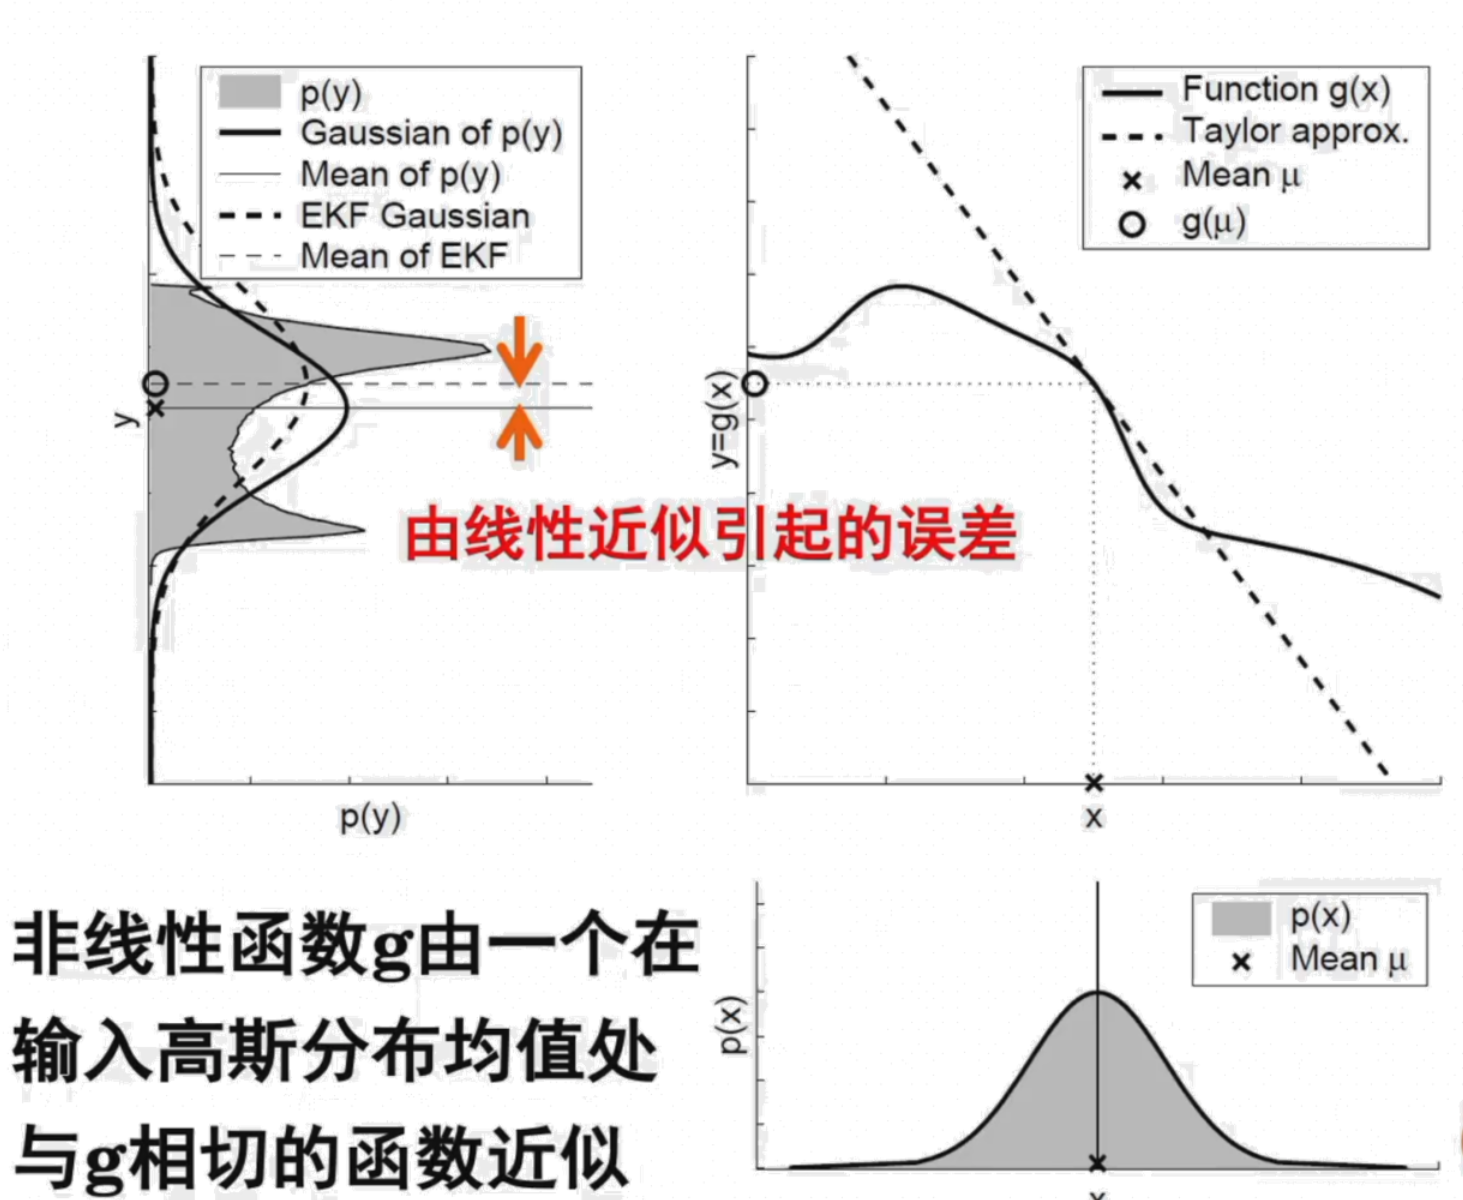
\includegraphics[width=0.6\linewidth]{images/ekf.png}
            \caption{线性近似}
        \end{figure}
        线性化的不确定程度来自于以下两个方面

        \begin{itemize}
            \item \textbf{自变量的不确定度}:如左图,自变量的不确定性较大,造成的误差就更大。
            \begin{figure}
                \centering
                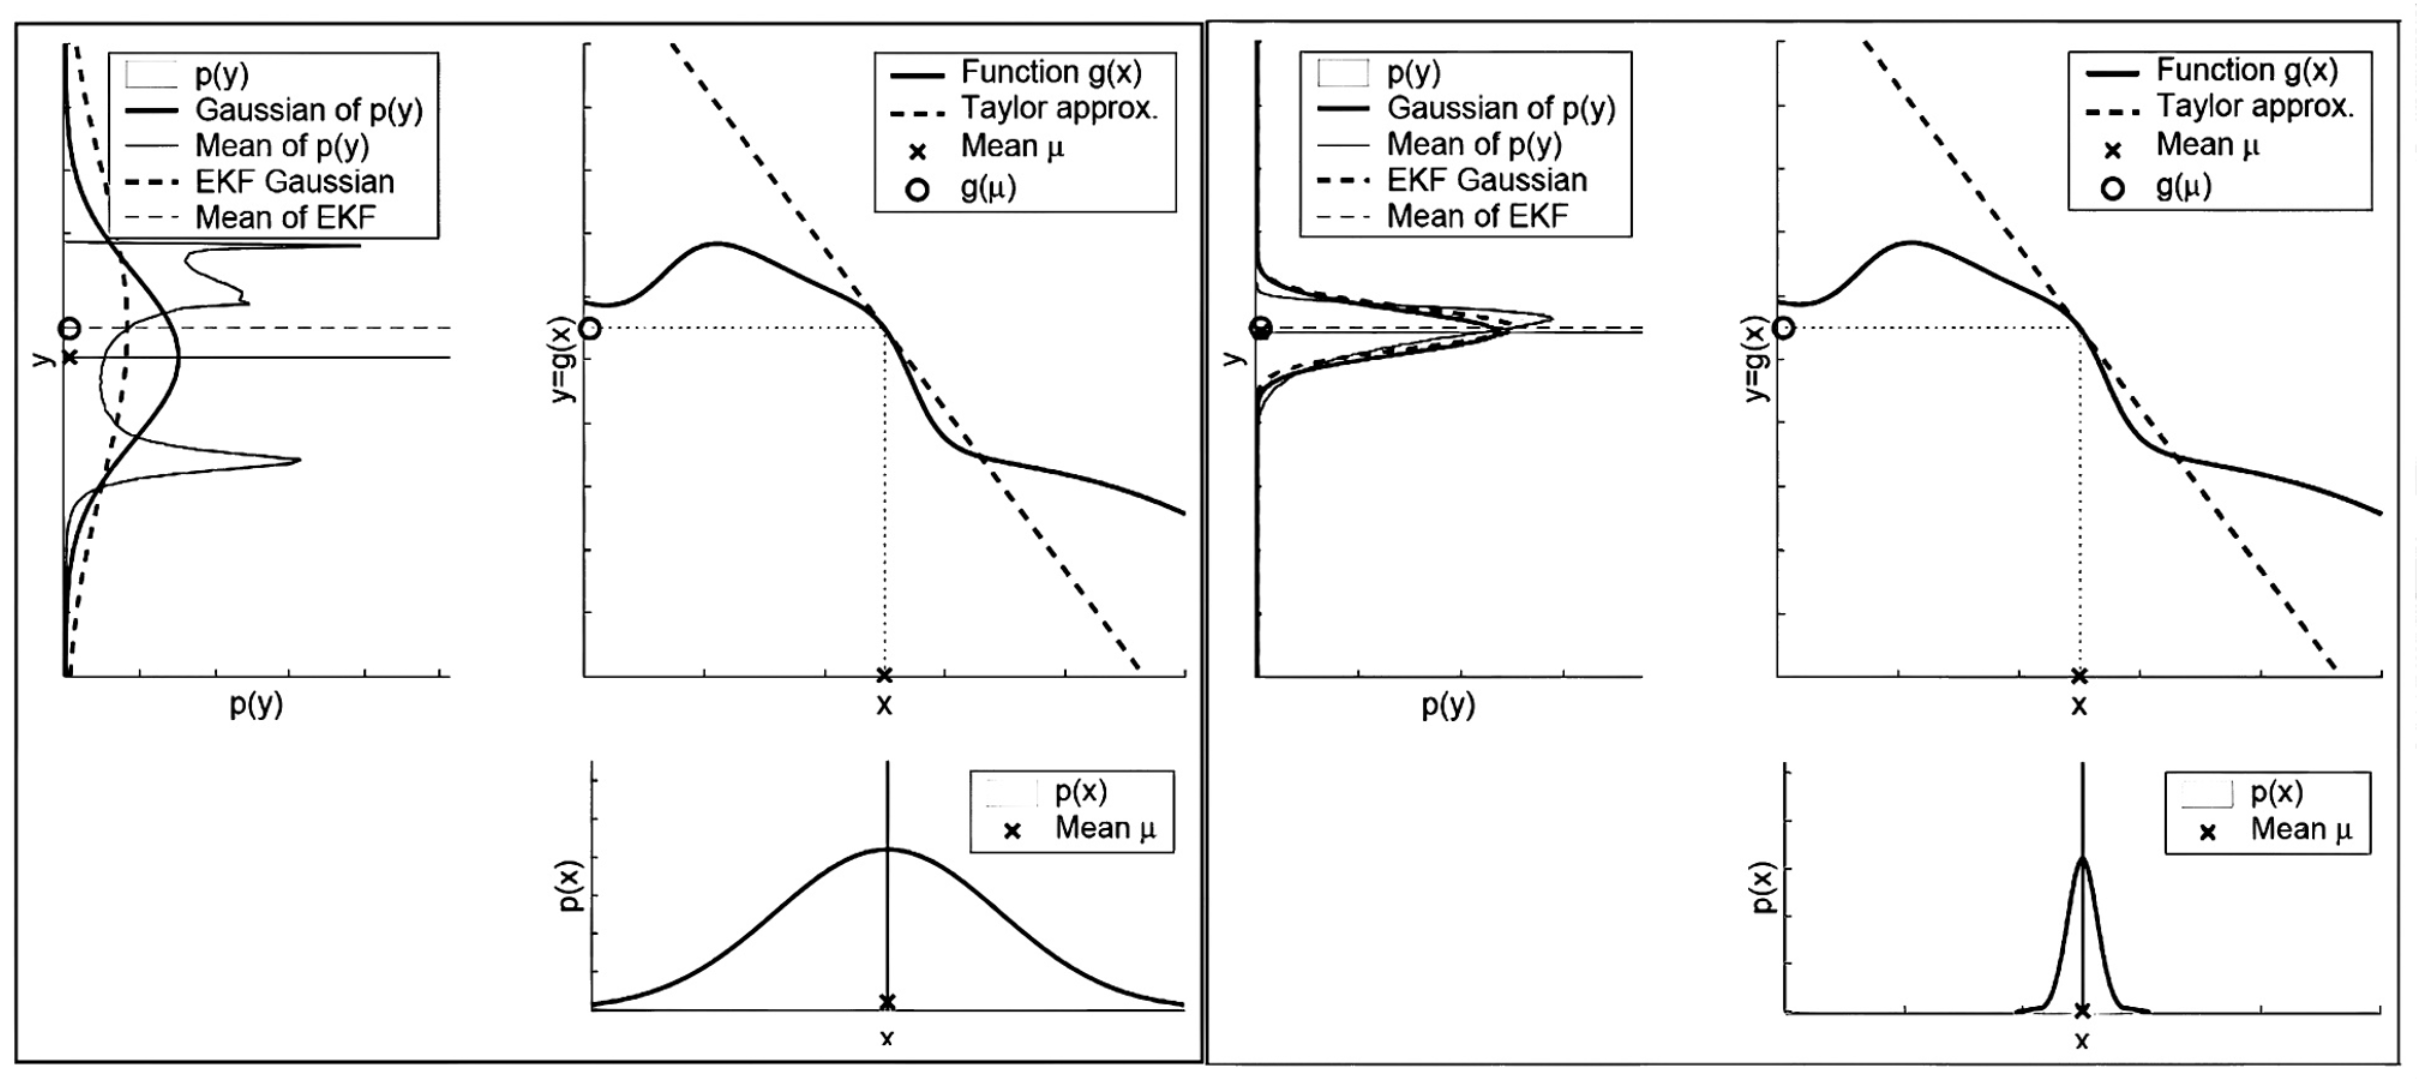
\includegraphics[width=0.5\linewidth]{images/xianxing1.png}
                \caption{自变量的不确定度影响}
            \end{figure}
            \item \textbf{局部非线性程度影响}:如左图,局部非线性程度较强,造成的误差就更大。
            \begin{figure}
                \centering
                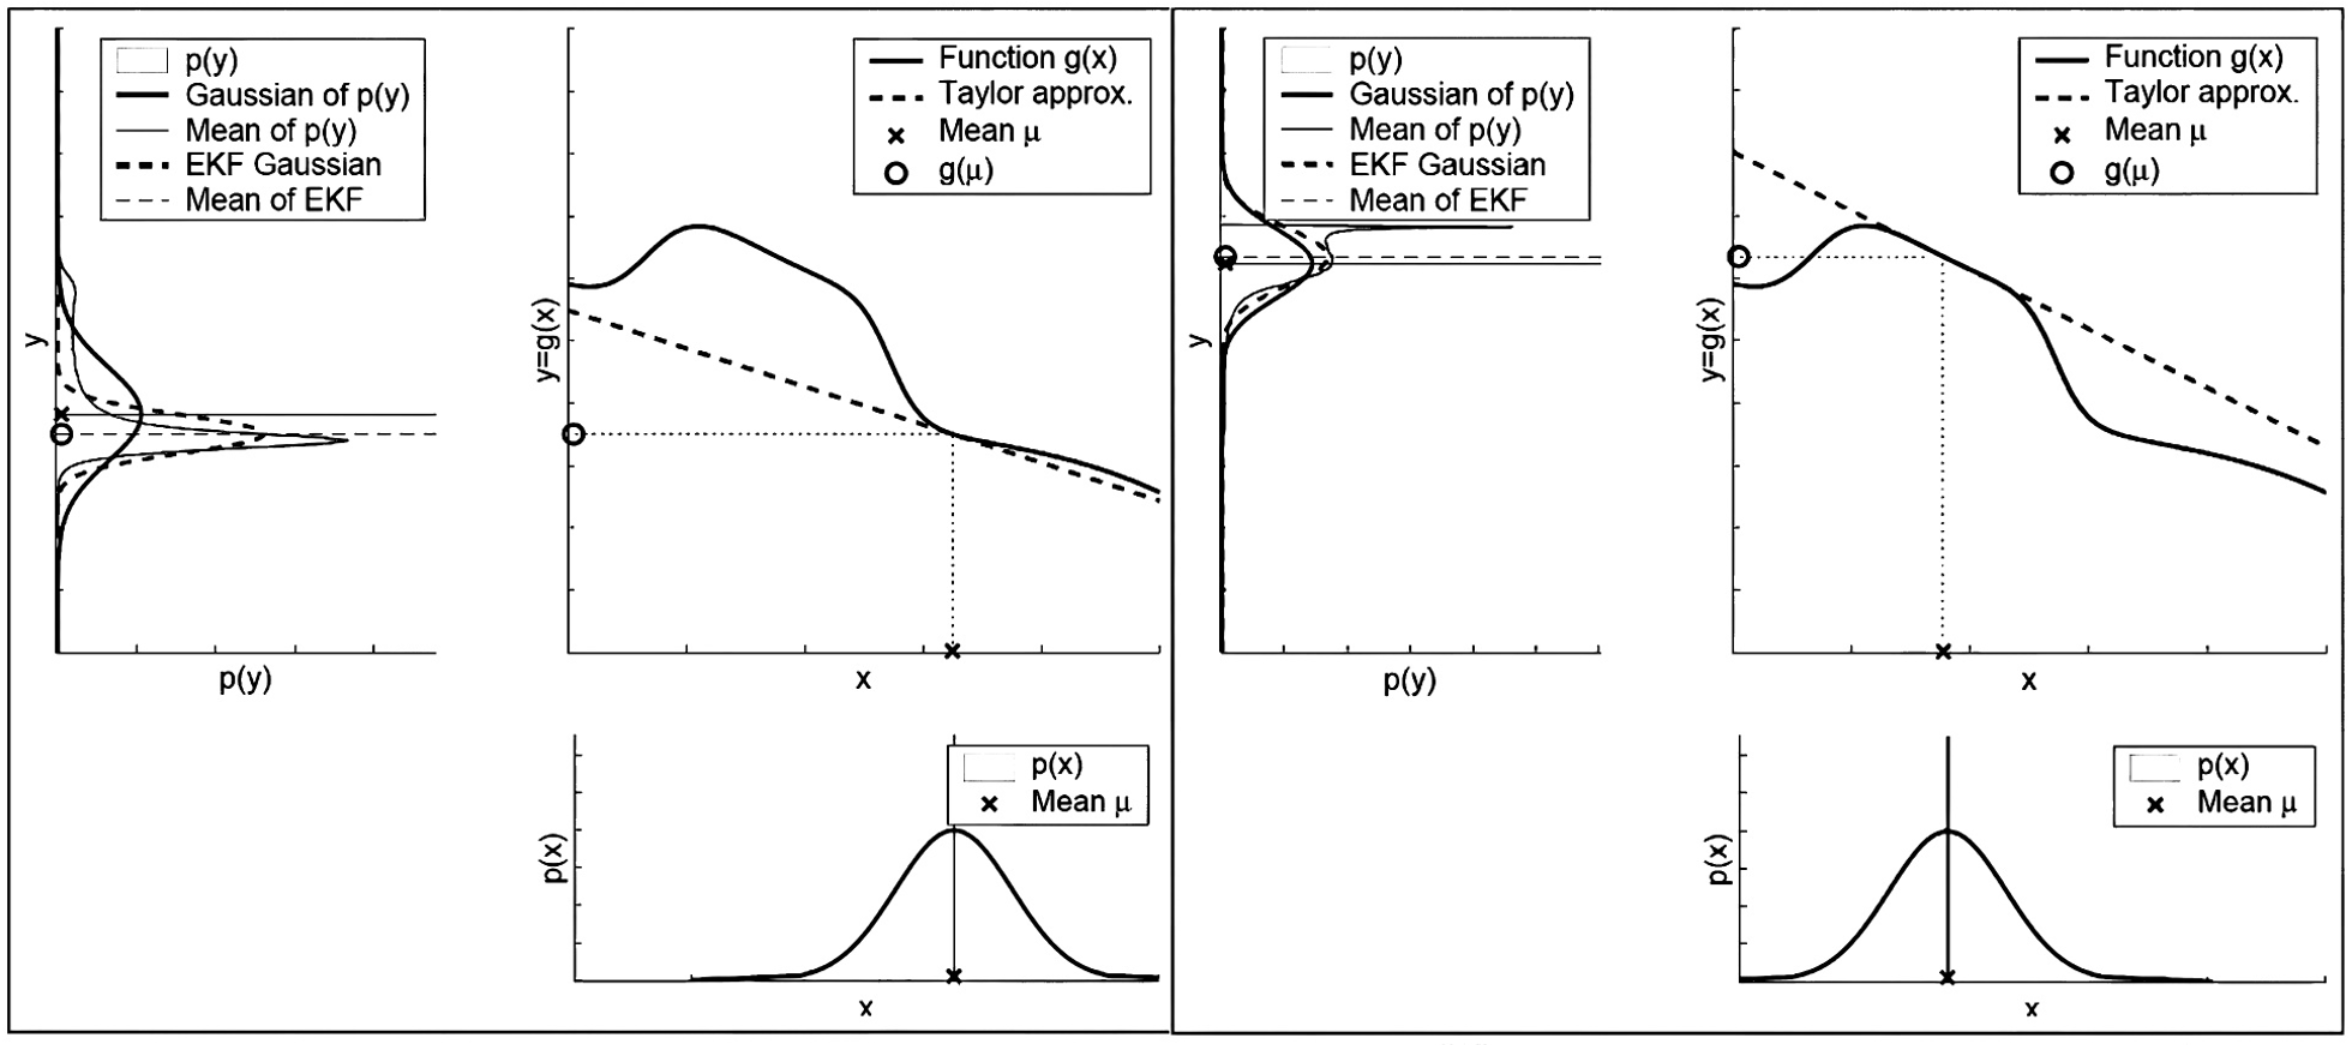
\includegraphics[width=0.5\linewidth]{images/xianxing2.png}
                \caption{局部非线性程度影响}
            \end{figure}
        \end{itemize}

        
  \item \textbf{EKF 算法公式} \ \ \ \ (\,$\boldsymbol{\mu}_{t-1},\ \boldsymbol{\Sigma}_{t-1},\ \mathbf{u}_{t-1},\ \mathbf{z}_t$\,)
  
  $$
  \bar{\boldsymbol{\mu}}_t \;=\; \textcolor{red}{g(\boldsymbol{\mu}_{t-1},\mathbf{u}_{t-1})}
  $$
  $$
  \bar{\boldsymbol{\Sigma}}_t \;=\; \mathbf{G}_t\,\boldsymbol{\Sigma}_{t-1}\,\mathbf{G}_t^\top \;+\; \mathbf{R}_t
  $$
  
  $$
  \mathbf{K}_t \;=\; \bar{\boldsymbol{\Sigma}}_t \,\mathbf{H}_t^\top \big(\mathbf{H}_t \bar{\boldsymbol{\Sigma}}_t \mathbf{H}_t^\top + \mathbf{Q}_t\big)^{-1}
  $$
  $$
  \boldsymbol{\mu}_t \;=\; \bar{\boldsymbol{\mu}}_t \;+\; \mathbf{K}_t\big(\mathbf{z}_t - \textcolor{red}{h(\bar{\boldsymbol{\mu}}_t)}\big)
  $$
  $$
  \boldsymbol{\Sigma}_t \;=\; \big[\mathbf{I} - \mathbf{K}_t \mathbf{H}_t\big]\ \bar{\boldsymbol{\Sigma}}_t
  $$
  $$
  \text{return}\ \ \boldsymbol{\mu}_t,\ \boldsymbol{\Sigma}_t
  $$
          计算$\mathbf{K}_t$时,时间复杂度是$O(k^{2.376})$,其中$k$是特征向量维度,即观测到的特征数\\
          计算$\boldsymbol{\Sigma}_t$时,时间复杂度是$O(n^2)$,其中$n$是状态向量维度,即机器人的位姿描述维度
  \item \textbf{推导过程}
  
  {\small\kaishu{
  \begin{enumerate}
    \item 运动方程(Motion model)
    
    $$
    \mathbf{x}_t \;=\; \textcolor{red}{g(\mathbf{x}_{t-1},\mathbf{u}_{t-1})} \;+\; \mathbf{v}_t,\qquad \mathbf{v}_t\sim\mathcal{N}(\mathbf{0},\mathbf{R}_t)
    $$
    
    取泰勒展开参数为 $\boldsymbol{\mu}_{t-1}$,有
    $$
    g(\mathbf{x}_{t-1},\mathbf{u}_{t-1}) \approx \textcolor{red}{g(\boldsymbol{\mu}_{t-1},\mathbf{u}_{t-1})} \;+\; \mathbf{G}_t(\mathbf{x}_{t-1}-\boldsymbol{\mu}_{t-1})
    $$
    $$
    \mathbf{G}_t \;=\; \left.\frac{\partial g(\mathbf{x}_{t-1},\mathbf{u}_{t-1})}{\partial \mathbf{x}_{t-1}}\right|_{\mathbf{x}_{t-1}=\boldsymbol{\mu}_{t-1}}
    \qquad\text{(Jacobian 矩阵, } n\times n\text{)}
    $$
    
    因而
    $$
    p(\mathbf{x}_t\mid \mathbf{x}_{t-1},\mathbf{u}_{t-1})
    \approx \mathcal{N}\big(\mathbf{x}_t;\ \textcolor{red}{g(\boldsymbol{\mu}_{t-1},\mathbf{u}_{t-1})} + \mathbf{G}_t(\mathbf{x}_{t-1}-\boldsymbol{\mu}_{t-1}),\ \mathbf{R}_t\big)
    $$
    
    \item 观测方程(Observation model)
    
    $$
    \mathbf{z}_t \;=\; \textcolor{red}{h(\mathbf{x}_t)} \;+\; \boldsymbol{\omega}_t,\qquad \boldsymbol{\omega}_t\sim\mathcal{N}(\mathbf{0},\mathbf{Q}_t)
    $$
    
    取泰勒展开参数为 $\bar{\boldsymbol{\mu}}_t$,有
    $$
    h(\mathbf{x}_t) \approx \textcolor{red}{h(\bar{\boldsymbol{\mu}}_t)} \;+\; \mathbf{H}_t(\mathbf{x}_t - \bar{\boldsymbol{\mu}}_t)
    $$
    $$
    \mathbf{H}_t \;=\; \left.\frac{\partial h(\mathbf{x}_t)}{\partial \mathbf{x}_t}\right|_{\mathbf{x}_t=\bar{\boldsymbol{\mu}}_t}
    \qquad\text{(Jacobian 矩阵, } k\times n\text{)}
    $$
    
    因而
    $$
    p(\mathbf{z}_t\mid \mathbf{x}_t)\approx \mathcal{N}\big(\mathbf{z}_t;\ \textcolor{red}{h(\bar{\boldsymbol{\mu}}_t)} + \mathbf{H}_t(\mathbf{x}_t-\bar{\boldsymbol{\mu}}_t),\ \mathbf{Q}_t\big)
    $$
    
    \item 状态预测(Prediction / Time update)
    
    $$
    \bar{p}(\mathbf{x}_t\mid \mathbf{Z}^{t-1},\mathbf{U}^{t-1})
    \;=\;\int p(\mathbf{x}_t\mid \mathbf{x}_{t-1},\mathbf{u}_{t-1})\; p(\mathbf{x}_{t-1}\mid \mathbf{Z}^{t-1},\mathbf{U}^{t-2})\ d\mathbf{x}_{t-1}
    $$
    
    使用上述线性化近似并代入 $\mathbf{x}_{t-1}\sim\mathcal{N}(\boldsymbol{\mu}_{t-1},\boldsymbol{\Sigma}_{t-1})$,得到高斯近似\footnote{两个高斯分布的卷积仍为高斯分布}:
    $$
    \bar{p}(\mathbf{x}_t\mid \mathbf{Z}^{t-1},\mathbf{U}^{t-1}) \;=\; \mathcal{N}\big(\mathbf{x}_t;\ \bar{\boldsymbol{\mu}}_t,\ \bar{\boldsymbol{\Sigma}}_t\big)
    $$
    其中
    $$
    \bar{\boldsymbol{\mu}}_t \;=\; \textcolor{red}{g(\boldsymbol{\mu}_{t-1},\mathbf{u}_{t-1})}
    $$
    $$
    \bar{\boldsymbol{\Sigma}}_t \;=\; \mathbf{G}_t\,\boldsymbol{\Sigma}_{t-1}\,\mathbf{G}_t^\top \;+\; \mathbf{R}_t
    $$
    
    \item 观测更新(Measurement update / Correction)
    
    先写贝叶斯更新:
    $$
    p(\mathbf{x}_t\mid \mathbf{Z}^t,\mathbf{U}^{t-1}) \;=\; \eta\; p(\mathbf{z}_t\mid \mathbf{x}_t)\; \bar{p}(\mathbf{x}_t\mid \mathbf{Z}^{t-1},\mathbf{U}^{t-1})
    $$
    
    将线性化的观测模型与预测高斯相乘并保持为高斯近似,得:
    $$
    p(\mathbf{x}_t\mid \mathbf{Z}^t,\mathbf{U}^{t-1}) \;=\; \mathcal{N}\big(\mathbf{x}_t;\ \boldsymbol{\mu}_t,\ \boldsymbol{\Sigma}_t\big)
    $$
    其中
    $$
    \mathbf{K}_t \;=\; \bar{\boldsymbol{\Sigma}}_t \,\mathbf{H}_t^\top \big(\mathbf{H}_t \bar{\boldsymbol{\Sigma}}_t \mathbf{H}_t^\top + \mathbf{Q}_t\big)^{-1}
    $$
    $$
    \boldsymbol{\mu}_t \;=\; \bar{\boldsymbol{\mu}}_t \;+\; \mathbf{K}_t\big(\mathbf{z}_t - \textcolor{red}{h(\bar{\boldsymbol{\mu}}_t)}\big)
    $$
    $$
    \boldsymbol{\Sigma}_t \;=\; \big[\mathbf{I} - \mathbf{K}_t \mathbf{H}_t\big] \bar{\boldsymbol{\Sigma}}_t
    $$
    
  \end{enumerate}
  }}
    \item \textbf{特点分析}:
    \begin{itemize}
        \item \textbf{优点}:
            \begin{itemize}
                \item 简单、计算高效
            \end{itemize}
        \item \textbf{缺点}:            
            \begin{itemize}
                \item 线性近似的好坏依赖于自变量的不确定程度、被近似函数局部非线性程度
                \item EKF采用多变量高斯分布表示估计的概率分布,这种单峰概率分布表示不适合于存在多个假设的情况
            \end{itemize}         
    \end{itemize}
    \item \textbf{EKF应用举例:}
    \\我们采用里程计运动模型和基于特征的观测模型,来进行一遍EKF流程:
  {\small\kaishu{
    \begin{enumerate}
    \item \textbf{运动模型}
    
    
    $$\mathbf{u}_{t-1}=(\delta_{rot1},\ \delta_{trans},\ \delta_{rot2})^T$$
    
    里程计运动模型
    $$\begin{pmatrix}x_t\\y_t\\\theta_t\end{pmatrix}=\begin{pmatrix}x_{t-1}+\hat{\delta}_{trans}\cos(\theta_{t-1}+\hat{\delta}_{rot1})\\y_{t-1}+\hat{\delta}_{trans}\sin(\theta_{t-1}+\hat{\delta}_{rot1})\\\theta_{t-1}+\hat{\delta}_{rot1}+\hat{\delta}_{rot2}\end{pmatrix}$$
    $$\hat{\delta}_{rot1}=\delta_{rot1}-\tilde{\delta}_{rot1}$$
    $$\hat{\delta}_{trans}=\delta_{trans}-\tilde{\delta}_{trans}$$
    $$\hat{\delta}_{rot2}=\delta_{rot2}-\tilde{\delta}_{rot2}$$
    $$\tilde{\delta}=(\tilde{\delta}_{rot1},\tilde{\delta}_{trans},\tilde{\delta}_{rot2})^T\sim\mathbf{N}(\mathbf{0},\mathbf{M}_t)$$
    其中
    $$\mathbf{M}_t=diag((\alpha_1\mid\delta_{rot1}\mid+\alpha_2\mid\delta_{trans}\mid)^2,(\alpha_3\mid\delta_{trans}\mid+\alpha_4\mid\delta_{rot1}+\delta_{rot2}\mid)^2,(\alpha_1\mid\delta_{rot2}\mid+\alpha_2\mid\delta_{trans}\mid)^2)$$


    但我们希望写成下面的形式:
    $$
    \mathbf{x}_t = g(\mathbf{x}_{t-1},\mathbf{u}_{t-1}) + \mathbf{v}_t
    $$
    即\footnote{这里我们给出的与前面讲到运动模型给出的形式不同,前面给出的形式是直接加上真值,所以没有$\mathbf{v}_t$这一项;这里我们写成测量值的形式,就有$\mathbf{v}_t$;可以理解为,前面的运动模型认为误差是发生在控制量上的,而此处给出的运动模型认为误差是发生在状态量上的。}:
    $$
    \begin{pmatrix} x_t\\ y_t\\ \theta_t \end{pmatrix}
    =
    \begin{pmatrix} x_{t-1}\\ y_{t-1}\\ \theta_{t-1} \end{pmatrix}
    +
    \begin{pmatrix}
      \delta_{trans}\ \cos(\theta_{t-1} + \delta_{rot1})\\[4pt]
      \delta_{trans}\ \sin(\theta_{t-1} + \delta_{rot1})\\[4pt]
      \delta_{rot1} + \delta_{rot2}
    \end{pmatrix}
    + \mathbf{v}_t
    $$
    $$
    \mathbf{v}_t = (\nu_x,\nu_y,\nu_\theta)^T \sim \mathcal{N}(0,\mathbf{R}_t)
    $$
    
    为此我们对我们原来的里程计运动模型进行改写,原来的里程计运动模型是
    $$
    \mathbf{x}_t = g(\mathbf{x}_{t-1},\mathbf{u}_{t-1} + \tilde{\delta})
    $$
    对该方程在 $\mathbf{u}_{t-1}$ 处作一阶泰勒展开,得
    \begin{align*}
    \mathbf{x}_t &= g\big(\mathbf{x}_{t-1},\,\mathbf{u}_{t-1} + \tilde{\delta}\big) \\
    &\approx g\big(\mathbf{x}_{t-1},\,\mathbf{u}_{t-1}\big)
           + g'\big(\mathbf{x}_{t-1},\,\mathbf{u}_{t-1}\big)\,\tilde{\delta} \\
    &= g\big(\mathbf{x}_{t-1},\,\mathbf{u}_{t-1}\big) + \mathbf{v}_t
    \end{align*}
    
    这样我们成功转化到EKF希望的运动模型形式了,我们可以求一下$\mathrm{v}_t$的协方差矩阵,可得
    $$
    \mathbf{R}_t = \mathbf{v}_t \mathbf{v}_t^T = g'(\mathbf{x}_{t-1},\mathbf{u}_{t-1})\,\tilde{\delta}\tilde{\delta}^T\, g'(\mathbf{x}_{t-1},\mathbf{u}_{t-1})^T
    = \mathbf{V}_t\,\mathbf{M}_t\,\mathbf{V}_t^T
    $$
    
    其中
    $$
    \mathbf{V}_t = \frac{\partial g(\mathbf{x}_{t-1},\mathbf{u}_{t-1})}{\partial \mathbf{u}_{t-1}}
    =
    \begin{pmatrix}
      \dfrac{\partial x_t}{\partial \delta_{rot1}} & \dfrac{\partial x_t}{\partial \delta_{trans}} & \dfrac{\partial x_t}{\partial \delta_{rot2}}\\[6pt]
      \dfrac{\partial y_t}{\partial \delta_{rot1}} & \dfrac{\partial y_t}{\partial \delta_{trans}} & \dfrac{\partial y_t}{\partial \delta_{rot2}}\\[6pt]
      \dfrac{\partial \theta_t}{\partial \delta_{rot1}} & \dfrac{\partial \theta_t}{\partial \delta_{trans}} & \dfrac{\partial \theta_t}{\partial \delta_{rot2}}
    \end{pmatrix}
    $$
    
    在具体代入时:
    $$
    \mathbf{V}_t =
    \begin{pmatrix}
      -\delta_{trans}\sin(\mu_{t-1,\theta} + \delta_{rot1}) & \cos(\mu_{t-1,\theta} + \delta_{rot1}) & 0\\[6pt]
      \delta_{trans}\cos(\mu_{t-1,\theta} + \delta_{rot1}) & \sin(\mu_{t-1,\theta} + \delta_{rot1}) & 0\\[6pt]
      1 & 0 & 1
    \end{pmatrix}
    $$
    \item \textbf{状态预测}
    至此,我们完成了运动模型的构建,可以由此进行位姿预估,即利用上一时刻的状态和控制量代入运动模型,得到预估的本时刻状态,其均值和方差应当是:
    $$
    \bar{\boldsymbol{\mu}}_t = g(\boldsymbol{\mu}_{t-1},\mathbf{u}_{t-1})
    $$
    $$
    \bar{\boldsymbol{\Sigma}}_t = \mathbf{G}_t \boldsymbol{\Sigma}_{t-1} \mathbf{G}_t^T + \mathbf{R}_t
    $$
    其中,$\mathbf{G}_t$是 $g(\mathbf{x}_{t-1},\mathbf{u}_{t-1})$ 的 Jacobian 矩阵
    $$
    \mathbf{G}_t = \frac{\partial g(\mathbf{x}_{t-1},\mathbf{u}_{t-1})}{\partial \mathbf{x}_{t-1}}\bigg|_{\mathbf{x}_{t-1}=\boldsymbol{\mu}_{t-1}}
    =
    \begin{pmatrix}
      \dfrac{\partial x_t}{\partial x_{t-1}} & \dfrac{\partial x_t}{\partial y_{t-1}} & \dfrac{\partial x_t}{\partial \theta_{t-1}}\\[6pt]
      \dfrac{\partial y_t}{\partial x_{t-1}} & \dfrac{\partial y_t}{\partial y_{t-1}} & \dfrac{\partial y_t}{\partial \theta_{t-1}}\\[6pt]
      \dfrac{\partial \theta_t}{\partial x_{t-1}} & \dfrac{\partial \theta_t}{\partial y_{t-1}} & \dfrac{\partial \theta_t}{\partial \theta_{t-1}}
    \end{pmatrix}
    =
    \begin{pmatrix}
      1 & 0 & -\delta_{trans}\sin(\mu_{t-1,\theta} + \delta_{rot1})\\[6pt]
      0 & 1 & \delta_{trans}\cos(\mu_{t-1,\theta} + \delta_{rot1})\\[6pt]
      0 & 0 & 1
    \end{pmatrix}
    $$

    
    \item \textbf{观测模型}\\
    同样,我们也希望写成:
    $$
    \mathbf{z}_t \;=\; h(\mathbf{x}_t) \;+\; \boldsymbol{\omega}_t,\qquad \boldsymbol{\omega}_t\sim\mathcal{N}(\mathbf{0},\mathbf{Q}_t)
    $$
    幸运的是,特征观测模型和这个形式是一致的,不用像运动模型再整理了
    $$
    \mathbf{m}=\{ \mathbf{m}_1,\mathbf{m}_2,\ldots,\mathbf{m}_N\},\qquad
    \mathbf{m}_i\ \text{在地图中的坐标为}\ (m_{ix},m_{iy})^T
    $$
    在时刻 $t$ 观测得到的特征为 $ \mathbf{z}_t = \{ z_t^1,z_t^2,\ldots\}$。每一个特征有一个 $c_t^i$ 说明 $z_t^i$ 在地图中对应特征,$c_t^i\in\{1,\ldots,N,N+1\}$。设 $c_t^i=j$,单个特征观测模型为
    $$
    z_t^i =
    \hat{z}_t^i = h(\mathbf{x}_t, c_t^i, \mathbf{m})
    + \omega,\qquad
    $$
    即
    $$
    z_t^i =
    \begin{pmatrix}
      \sqrt{(m_{jx}-x)^2 + (m_{jy}-y)^2} \\[6pt]
      \mathrm{arctan2}(m_{jy}-y,\; m_{jx}-x) - \theta \\[6pt]
      s_j
    \end{pmatrix}
    + \omega
    $$
    其中
    $$\omega_t \sim \mathcal{N}(0,\mathbf{Q}_t)$$
    求 $h(\mathbf{x}_t, c_t^i, \mathbf{m})$ 的 Jacobian 矩阵:
    $$
    \mathbf{H}_t^i = \frac{\partial h(\mathbf{x}_t, c_t^i, \mathbf{m})}{\partial \mathbf{x}_t}\bigg|_{\mathbf{x}_t=\bar{\boldsymbol{\mu}}_t}
    $$
    
    \item \textbf{观测更新(基于所有观测特征的位姿更新)}
    $$
    p(\mathbf{z}_t \mid \mathbf{x}_t, \mathbf{c}_t, \mathbf{m}) = \prod_i p(z_t^i \mid \mathbf{x}_t, c_t^i, \mathbf{m})
    $$
    $$
    p(\mathbf{x}_t \mid Z^t, U^{t-1}, \mathbf{m}) = \mathcal{N}\big(\mathbf{x}_t;\ \boldsymbol{\mu}_t,\ \boldsymbol{\Sigma}_t\big)
    $$
    $$
    \boldsymbol{\mu}_t = \bar{\boldsymbol{\mu}}_t + \sum_i \mathbf{K}_t^i\big(z_t^i - h(\bar{\boldsymbol{\mu}}_t, c_t^i, \mathbf{m})\big)
    $$
    $$
    \boldsymbol{\Sigma}_t = \big[\mathbf{I} - \sum_i \mathbf{K}_t^i \mathbf{H}_t^i\big]\ \bar{\boldsymbol{\Sigma}}_t
    $$
    
    
  \end{enumerate}
  }}
    \begin{figure}[H]
        \centering
        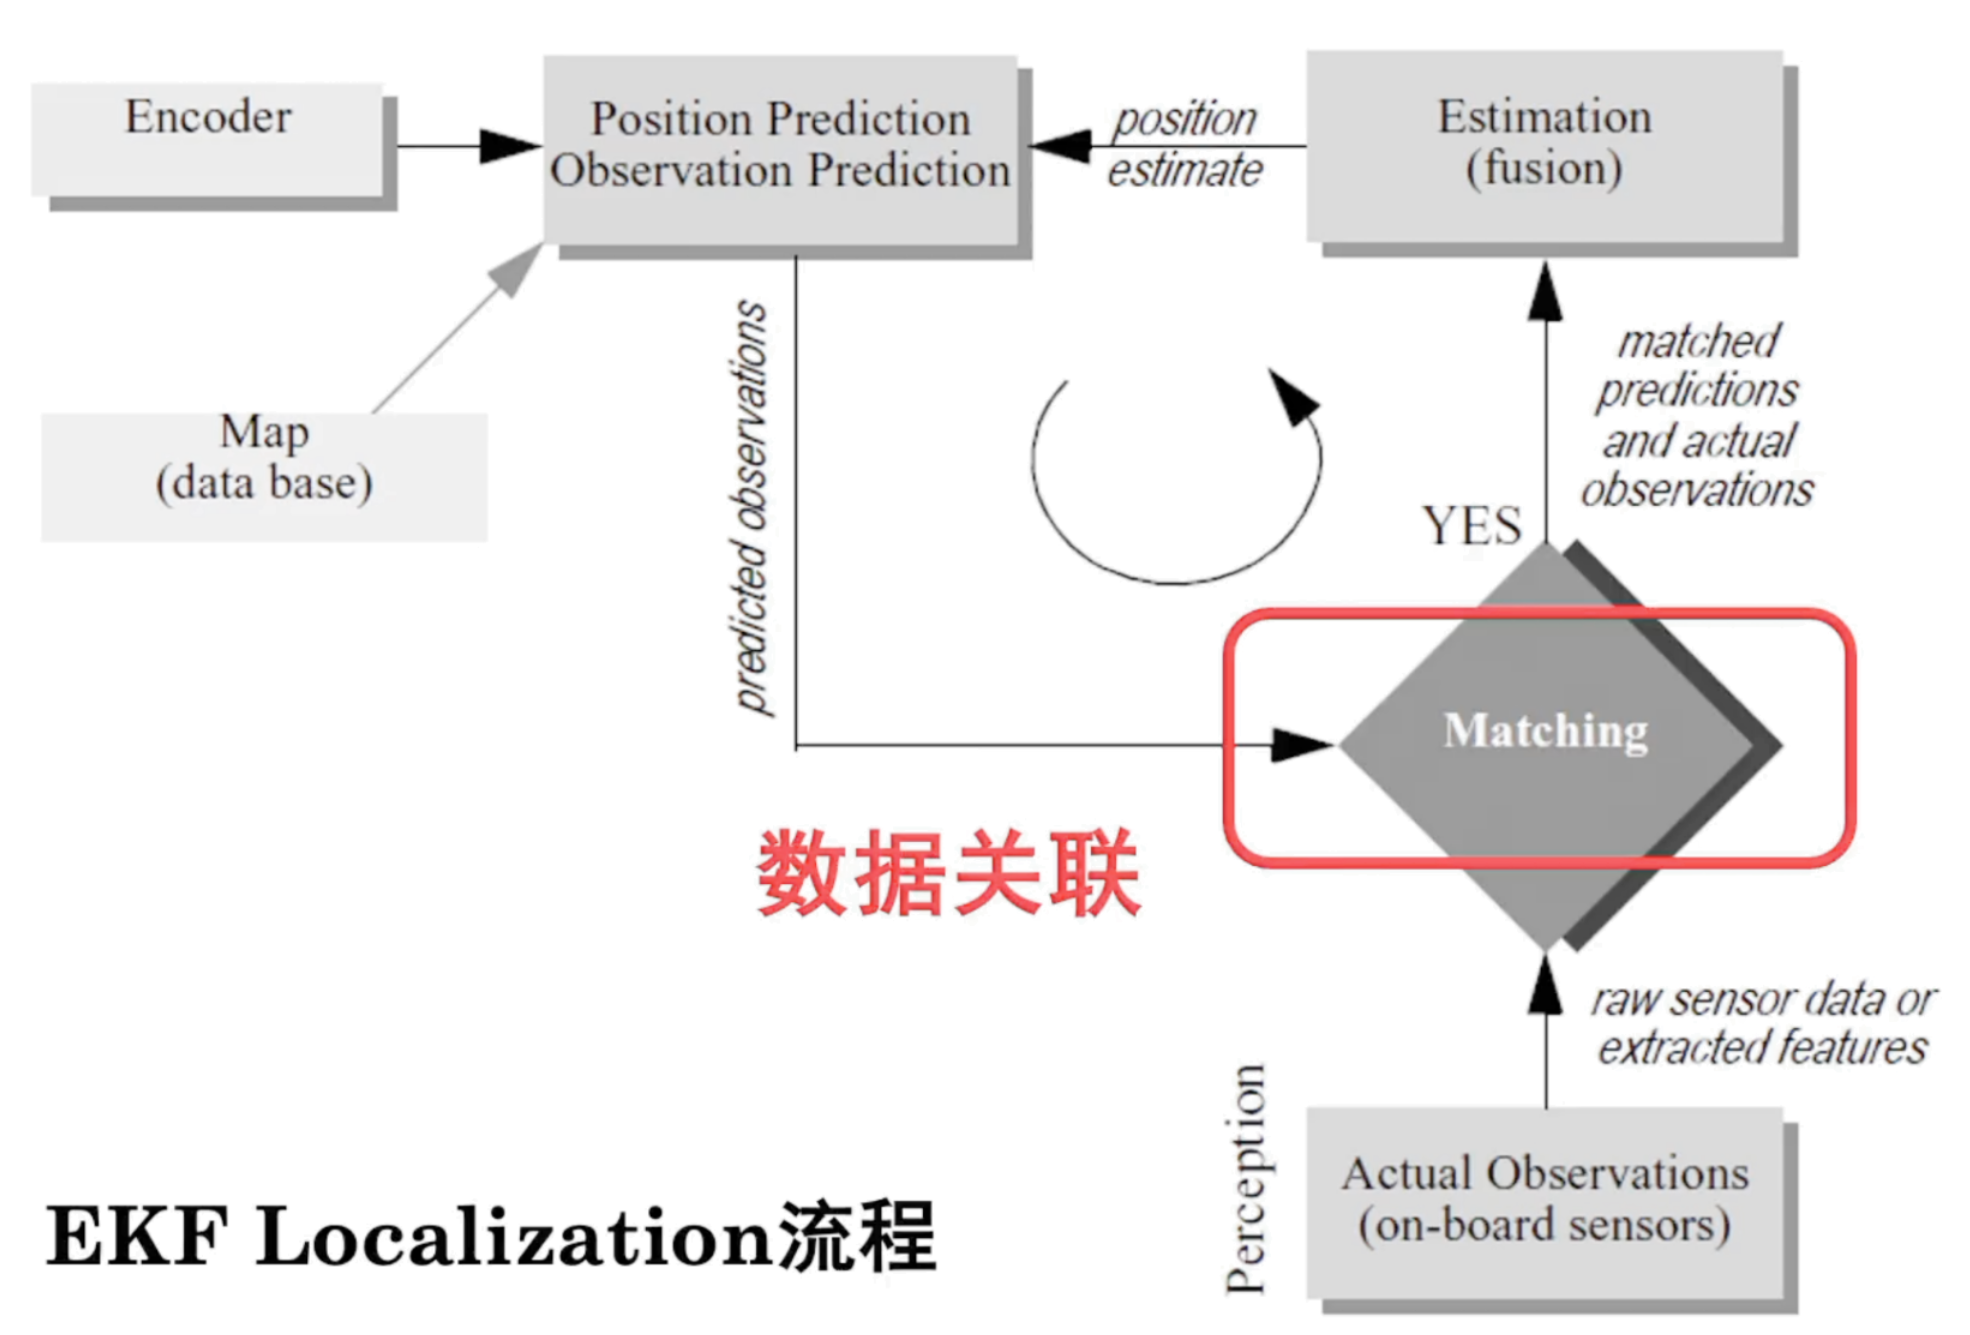
\includegraphics[width=0.5\linewidth]{images/ekf_pipeline.png}
        \caption{EKF定位流程}
    \end{figure}
    \item \textbf{数据关联问题}
    \begin{itemize}
    \begin{figure}[H]
        \centering
        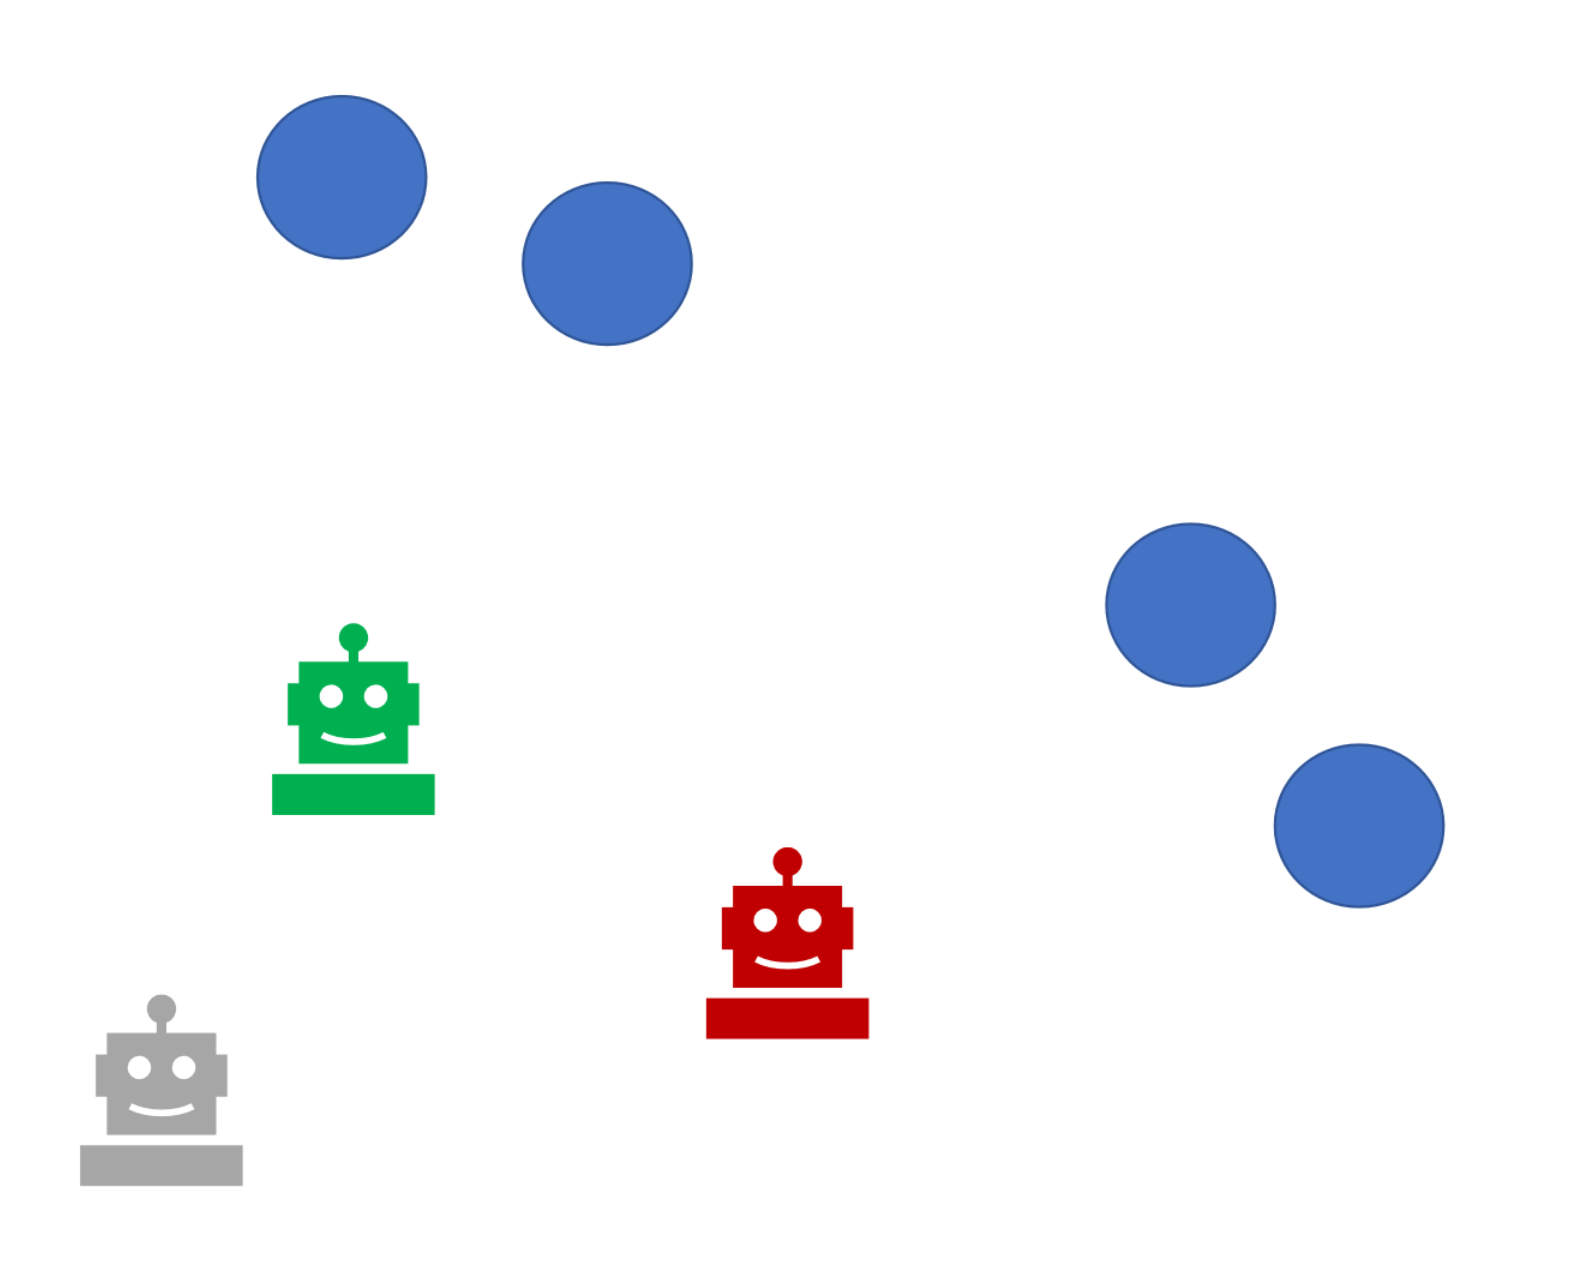
\includegraphics[width=0.5\linewidth]{images/data_connection.png}
        \caption{我随手画的一个草图:机器人上一时刻在灰色位置,下一时刻实际上运行到了绿色位置,但是运动模型估计出现较大误差,让机器人以为自己到了红色位置,此时用观测模型修正,自以为在红色位置的机器人发现眼前有两个物体,和绿色位置能看到的一致,让机器人更加坚定了自己错误的信念}
    \end{figure}
        \item \textbf{问题}:一般情况下$c^i_t$未知
        \item \textbf{解决办法}:maximum likelihood correspndence
        $$\hat{c}_t = \arg\max_{c_t} p(\mathbf{z}_t | C^t, \mathbf{m}, \mathbf{Z}^{t-1}, \mathbf{U}^{t-1})$$
        为避免指数级的巨大计算量,单独估计每个特征的最大可能对应
        $$
        \hat{c}_t^i = \arg\max_{c_t^i} p(\mathbf{z}_t^i | C^t, \mathbf{m}, \mathbf{Z}^{t-1}, \mathbf{U}^{t-1})$$
        $$\approx \arg\max_{c_t^i} \mathscr{N} \left( \mathbf{z}_t^i; h(\bar{\mathbf{\mu}}_t, c_t^i, \mathbf{m}), \mathbf{H}_t^i \bar{\mathbf{\Sigma}}_t \mathbf{H}_t^{iT} + \mathbf{Q}_t \right)$$
    \end{itemize}

    
\end{enumerate}
\subsection{粒子滤波定位法(PF)}
\end{document}